\chapter{L2MuonSAにおけるNSWを用いた横運動量再構成アルゴリズムの動作検証と改良}\label{chapter5}
%本章ではNSWを用いたL2MuonSA部分飛跡再構成アルゴリズムについて、Run-3実データを用いた性能評価の結果について述べ、さらに検討したヒット選択アルゴリズムの説明および性能評価について述べる。


本章では、まず先行研究(\cite{article:kumaoka}, \cite{article:noguchi})において開発されたNSW部分飛跡再構成アルゴリズムについて紹介し、実データでの性能を評価した結果について述べる。
評価の結果~NSWの検出器ヒットの一部が部分飛跡の再構成に用いられないことが多いことが分かった。
これを回復するアルゴリズムを考案しRun-3実データにおいて現行のアルゴリズムとの性能を比較した結果について述べる。

\newpage

\section{NSWを用いたL2MuonSA部分飛跡再構成アルゴリズム}\label{chapter5-1}
第2章で述べたのように~NSWは~sTGC8層と~MM8層の合計16層から構成される。

NSWを用いたL2MuonSAアルゴリズムでは、まず~sTGC、MMでそれぞれヒットの選別を行い、選ばれた~sTGC、MMのヒットを組み合わせて部分飛跡が再構成され~SPが作成される。
以下では~sTGC、MMそれぞれでのヒット選択アルゴリズムと、ヒットを組み合わせて~SPを作成するアルゴリズムについて説明する。

\subsection{NSWの各検出器におけるヒット選択アルゴリズム}\label{chapter5-1-1}
\subsubsection{sTGCヒット選択アルゴリズム}
sTGCでは、ストリップが幅が小さいため1つの荷電粒子が通過すると複数のストリップで反応を起こす。この複数反応したストリップから読み出された電荷などの情報を用いて、1つの荷電粒子が通過した位置を求めるクラスタリングを行う。
以下のヒット選択アルゴリズムではクラスタリング後のヒット情報を用いる。
第3章で述べたように~L1の情報を用いてミドルステーションから定義されたロードの情報を用いて、ロード内にある~sTGCのヒットを選び、さらに~sTGCヒット選択アルゴリズムを用いて~NSWでの~SPの再構成に用いる~sTGCヒットを選択する。

図~\ref{fig:5-1}は~sTGCヒット選択アルゴリズムの概要図である。

\begin{figure}[H]
  \centering
  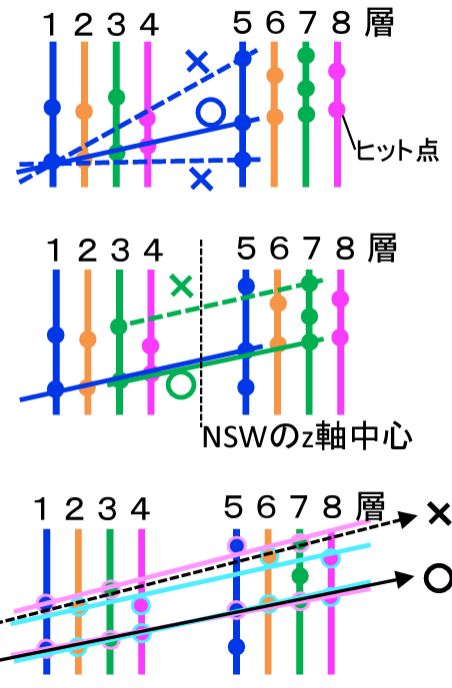
\includegraphics[clip, width=6cm]{fig/5/sTGC_hitSelectAlg.png}
  \caption{L2MuonSAにおけるsTGCヒット選択アルゴリズムの概要図\cite{article:kumaokaJPS}。}
  \label{fig:5-1}
\end{figure}

sTGCヒット選択アルゴリズムの流れを以下に示す。
\begin{enumerate}
    \item $i$層目と$i+4$層目~($i=1, 2, 3, 4$)のヒットをペア1にし、ペア1を結ぶ直線の傾きの絶対値が0.14rad以下あるいは0.6rad以上あるペア1を除外する。また切片が原点から300mm以上離れているペア1も除外する。またペア1に1つしかヒットがない場合、原点と片方のヒットでペア1を作成する。
    \item 1で残ったペア1に対して、奇数層目同士~((1層目, 5層目), (3層目, 7層目))、偶数層目同士~((2層目, 6層目), (4層目, 8層目))でペア2を作る。この際、$z$軸に垂直でNSWの中心を通る平面においてペア1の直線同士の距離が50mm以上離れているペア2は除外する。
    \item 2で作成したペア2を組み合わせて、最大8つのヒットで構成されるペア3を作成する。この時に$z$軸に垂直でNSWの中心を通る平面においてペア2の直線同士の距離が100mm以上離れているペア3は除外する。またペア2の切片の平均値の絶対値が100mm以上のペア3も除外する。
    \item ペア3の中で、以下の式で表される位置のばらつき$s$が最小の組み合わせを選択する。
    \begin{equation}
        s=\frac{1}{n-2} \sum_{i=1}^n\left(\hat{y}_i-y_i\right)^2\label{equ5-1}
    \end{equation}
    ここで$n$は組み合わせの中にあるヒット数、$y_i$は各ヒットの$R$座標、$\hat{y}_i$は組み合わせを最小二乗法によりフィットした直線の各層の$z$座標における$R$座標である。
\end{enumerate}

上記で選ばれた最大8つの~sTGCヒットを~MMのヒットと組み合わせて~SPの再構成に用いる。

\subsubsection{MMヒット選択アルゴリズム}
第2章で述べたように~MMにはストリップが底面に平行な~$X$層と$\pm15^\circ$傾けて配置された~$U$~($V$)層がある。
$X$層、$U$層、$V$層は図~\ref{fig:2-26}の順に並べられている。

sTGCと同様に~MMのヒットもクラスタリング後のヒット情報を用いて、ミドルステーションから定義されたロード内のヒットを選び、さらに~MMヒット選択アルゴリズムを用いて~NSWでの~SPの再構成に用いる~MMヒットを選択する。

MMヒット選択アルゴリズムの流れを以下に示す。
\begin{enumerate}
    \item $X$層(1層目, 7層目)、$X$層(2層目, 8層目)、$U$層(3層目, 5層目)、$V$層(4層目, 6層目)のヒットでペア1を作成し、ペア1を結ぶ直線の傾きの絶対値が0.1rad以下あるいは0.7rad以上あるペア1を除外する。また切片が原点から500mm以上離れているペア1も除外する。またペア1に1つしかヒットがない場合、原点と片方のヒットでペア1を作成する。また2つのペア1の切片の平均値の絶対値が200mm以上のペア2も除外する。
    \item 1で残ったペア1に対して、$X$層同士~((1層目, 7層目), (2層目, 8層目))、でペア2を作成する。この際、$z$軸に垂直でNSWの中心を通る平面においてペア1の直線同士の距離が50mm以上離れているペア2は除外する。
    \item $U$層と$V$層~((3層目, 5層目), (4層目, 6層目))でペア2を作る。3層目、4層目と5層目、6層目でそれぞれ$\phi$の差を取り、どちらかで0.05rad以上の差があった場合は除外する。差が小さければ、両ペアの平均をとる。$U$、$V$層における$\phi$の計算については~\ref{chapter5-1-2}で述べる。
    \item 2と3で作成したペア2を組み合わせて、最大8つのヒットで構成されるペア3を作成する。また後述する方法で求めた$\phi$の情報を用いて各層の$R$座標を補正する。補正された$R$座標~($R'$)と$z$座標を用いてペア3の部分飛跡を再構成し、\eqref{equ5-1}式で表される位置のばらつき$s$が最小の組み合わせを選択する。
\end{enumerate}

このアルゴリズムで選ばれた最大8つの~MMのヒットを~sTGCのヒットと組み合わせて~SPの再構成に用いる。


\subsection{sTGCとMMのヒット組み合わせによるNSW部分飛跡再構成}\label{chapter5-1-2}
ヒット選択アルゴリズムで選択された~sTGC、MMヒットを組み合わせて~NSWでの~SPを再構成する。
sTGC~strip層と~MM~$X$層はチェンバー中心におけるストリップのビーム軸からの距離$R$しか分からない。
sTGC~wireや~MM~stereo~layerの情報を組み合わせて$\phi$情報を計算し、実際に検出器をミューオンが通過した位置とビーム軸との距離$R'$に補正を行う。
$R$から$R'$への補正の方法を以下に示す。

\begin{enumerate}
    \item sTGCと~MM~$X$層のヒットの~($z$, $R$)座標を最小二乗法を用いて直線でフィットを行う。
    \item sTGC~wireの情報を用いて、各層の$\phi$を求める。1で定義した直線の~sTGC~wireの各層の$z$座標での$R$座標を求め$R_{{\rm{Int}},i}$とする。$R_{{\rm{Int}},i}$を用いて、式\eqref{equ5-2}で$\phi_{{\rm{sTGC}},i}$を求める。
    \begin{equation}
        \phi_{\mathrm{sTGC},i}=\arctan\left(\frac{R_{\mathrm{wire},i}}{R_{\mathrm{int},i}} \times \tan(\phi_{\mathrm{wire},i})\right)\label{equ5-2}
    \end{equation}
    ここで$R_{{\rm{wire}},i}$と$\phi_{{\rm{wire}},i}$はそれぞれ各ヒットがあるワイヤの中心の$R$、$\phi$座標である。変数の定義を図~\ref{fig:5-2}に示す。
    
    \begin{figure}[H]
        \centering
        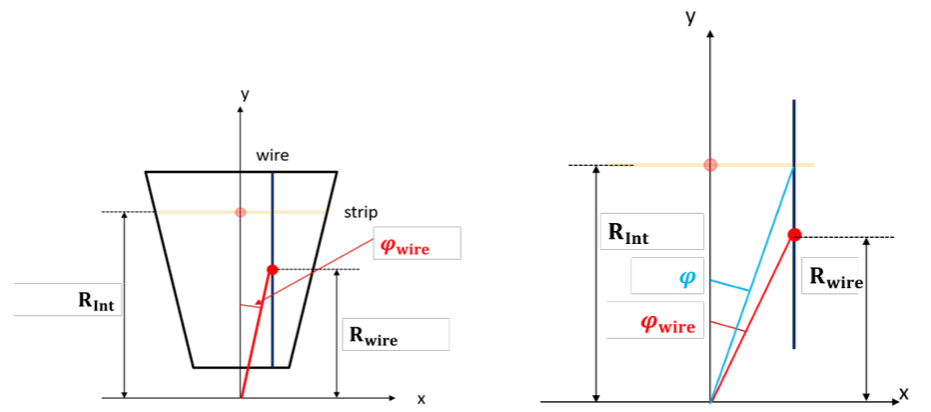
\includegraphics[clip, width=12cm]{fig/5/sTGC_phi.png}
        \caption{sTGCにおける$\phi$の計算\cite{article:noguchi}。}
        \label{fig:5-2}
    \end{figure}
        
    \item MM~stereo~layerの情報を用いて、$\phi_{{\rm{MM}},i}$を求める。sTGC~wireの時と同様に1で定義した直線の~MM~stereo~layerの各層の$z$座標での$R$座標を求め$R_{{\rm{Int}},i}$とする。
    $U$、$V$層はそれぞれ$\pm1.5^{\circ}$ずつ傾けて配置されているので、$x-y$平面での$U$層~($X$層)の交点の$x$座標$x_{{\rm{U}},i}$~($x_{{\rm{V}},i}$)を以下の式で定義する。
    \begin{equation}
        x_{\mathrm{U},i}=\frac{R_{\mathrm{U},i}-R_{\mathrm{Int},i}}{\tan(\frac{\pm1.5}{360}) \times 2\pi}\label{equ5-3}
    \end{equation}
    $x_{{\rm{U}},i}$を用いて、以下の式で$\phi_{{\rm{MM}},i}$を求める。
    
    \begin{equation}
        \phi_{\mathrm{MM},i}=\arctan\left(\frac{x_{\mathrm{U},i}}{R_{\mathrm{Int},i}}\right)\label{equ5-4}
    \end{equation}
    \begin{figure}[H]
        \centering
        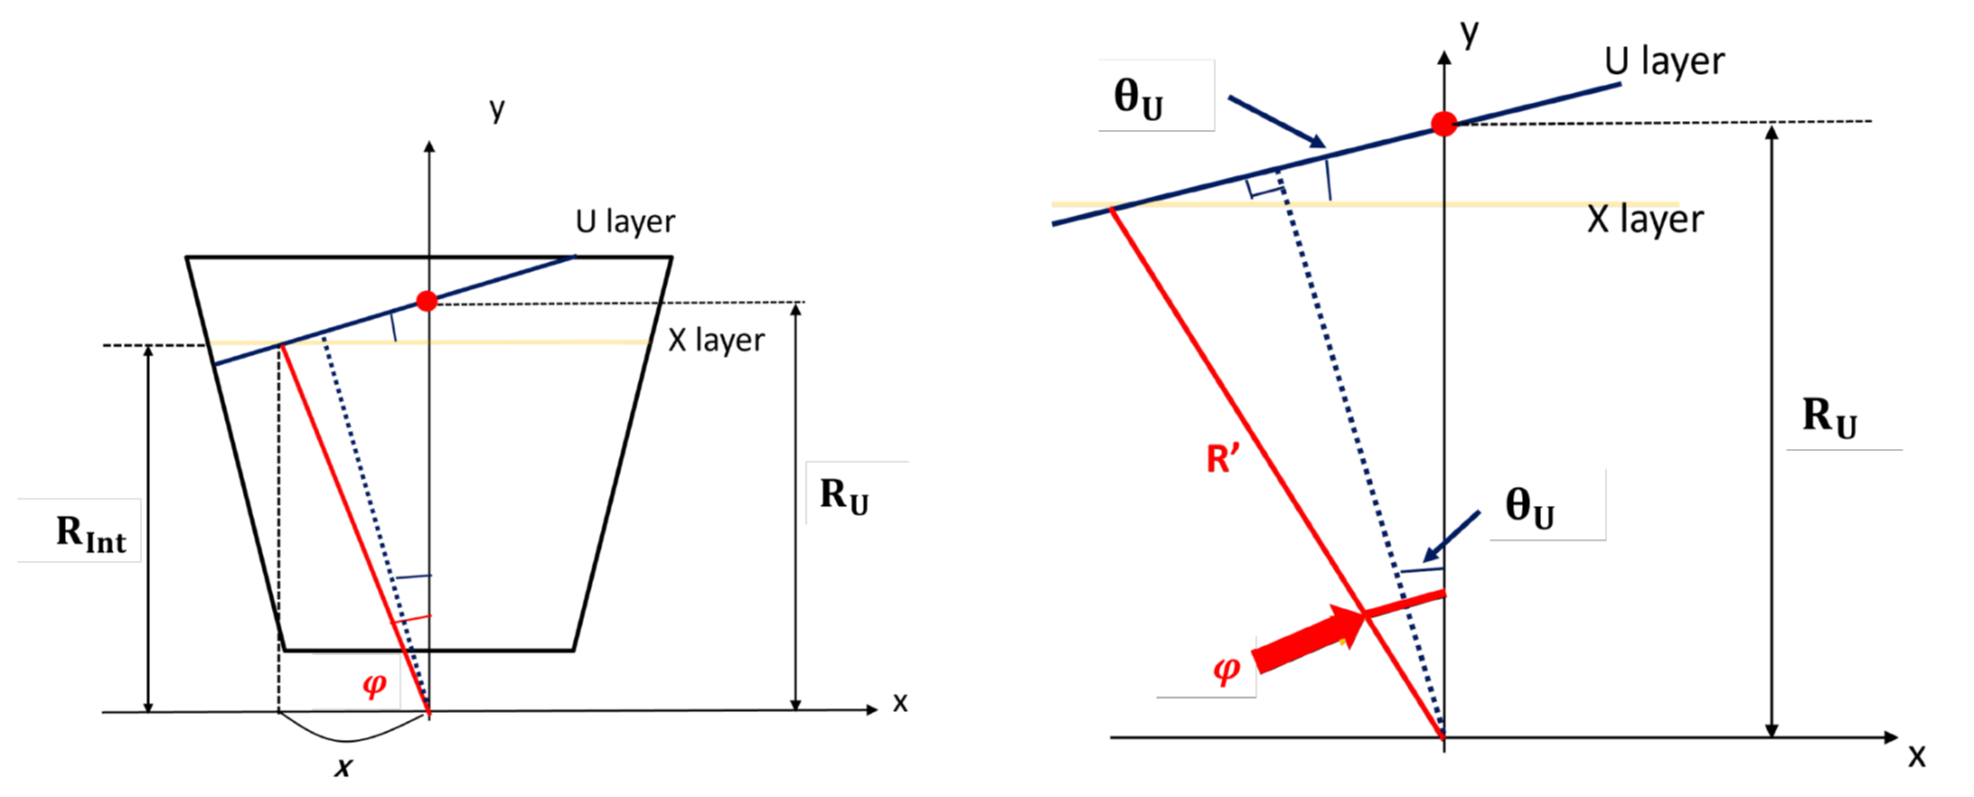
\includegraphics[clip, width=12cm]{fig/5/mm_phi.png}
        \caption{MMにおける$\phi$の計算と$U$層における$\phi$の射影\cite{article:noguchi}。}
        \label{fig:5-3}
    \end{figure}
    \item 2と3で求めた各層の$\phi$の平均値$\phi_{\rm{Avg}}$を計算し、sTGC~stripや~MM~$X$層の各層での$R$を$\cos(\phi_{\rm{Avg}})$で割ることによって実際のヒットの$R$座標である$R'$を求める。
    \begin{equation}
        R'=\frac{R}{\cos(\phi_{\mathrm{Avg}})}\label{equ5-5}
    \end{equation}
    MMの~stereo~layerでは$\phi_{\mathrm{MM}}$を用いて式~\eqref{equ5-7}で射影して$R'$を求める。
    \begin{equation}
        R' \times \cos(\phi_{\mathrm{U}}-\theta_{\mathrm{U}})=R_{\mathrm{U}} \times \cos(\theta_{\mathrm{U}})\label{equ5-6}
    \end{equation}
    \begin{equation}
    \begin{split}
        R' &= \frac{R_{\mathrm{U}} \times \cos(\theta_{U})}{\cos(\phi_{\mathrm{U}}-\theta_{\mathrm{U}})}\\
        &= \frac{R_{\mathrm{U}} \times \cos(\theta_{U})}{\cos(\phi_{\mathrm{U}})\cos(\theta_{\mathrm{U}}) + \sin(\phi_{\mathrm{U}})\sin(\theta_{\mathrm{U}})}\label{equ5-7}
    \end{split}
    \end{equation}
\end{enumerate}

\section{NSWを用いた横運動量の計算方法}\label{chapter5-2}
NSWはインナーステーションに配置されているので、NSWの~SPを~L2MuonSAでの$\pt$再構成に用いる場合は角度$\beta$を用いる。
角度$\beta$から$\pt$を求める方法は、第3章で述べたように~LUTを用いる。
以下の図は~NSWの~SPを用いた角度$\beta$の定義を表す。
\begin{figure}[H]
    \centering
    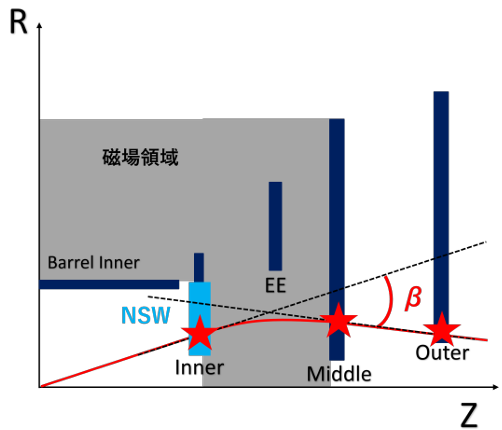
\includegraphics[clip, width=8cm]{fig/5/NSW_beta.png}
    \caption{NSWを用いた$\beta$の定義\cite{article:noguchi}}
    \label{fig:5-4}
\end{figure}

\section{Run-3実データにおけるNSWを用いたL2MuonSAの性能評価}\label{chapter5-3}

L2MuonSAで~NSWを用いた時の$\pt$の精度を評価するための変数として、以下の式~\eqref{equ5-8}で表される$\pt$~residualと~SPとインナーステーションにおけるオフラインセグメントの傾きの差である$\Delta\theta$(式~\eqref{equ5-9})を用いた。

\begin{equation}
    \pt~\mathrm{residual}= \frac{1/p_{\mathrm{T,L2SA}} - 1/p_{\mathrm{T,offline}}}{1/p_{\mathrm{T,offline}}}\label{equ5-8}
\end{equation}

\begin{equation}
    \Delta \theta = \theta_{\mathrm{L2MuonSA, SP}} - \theta_{\mathrm{offline}}\label{equ5-9}
\end{equation}

$\Delta \theta$の定義を図~\ref{fig:5-7}に示す。
\begin{figure}[H]
    \centering
    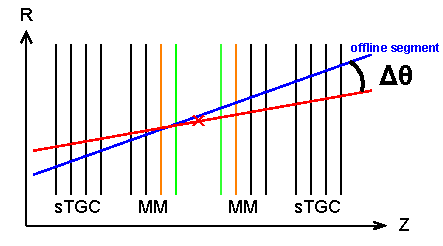
\includegraphics[clip, width=8cm]{fig/5/deltaTheta.pdf}
    \caption{$\Delta \theta$の定義}
    \label{fig:5-7}
\end{figure}

Run-3実データとモンテカルロシミュレーションにおいて~NSWを$\pt$再構成に用いる~L2MuonSAアルゴリズムを走らせたときの、$\pt$~residualと$\Delta\theta$の分布を図~\ref{fig:ptresidualDataMC}と\ref{fig:deltaThetaDataMC}に示す。
またL2MuonSAで$alpha$、$beta$からそれぞれ求めた$p_{\rm{T, \alpha}}$、$p_{\rm{T, \beta}}$~residual分布を図~\ref{fig:ptresidualAlphaBeta}に示す。

\begin{figure}[H]
    \centering
    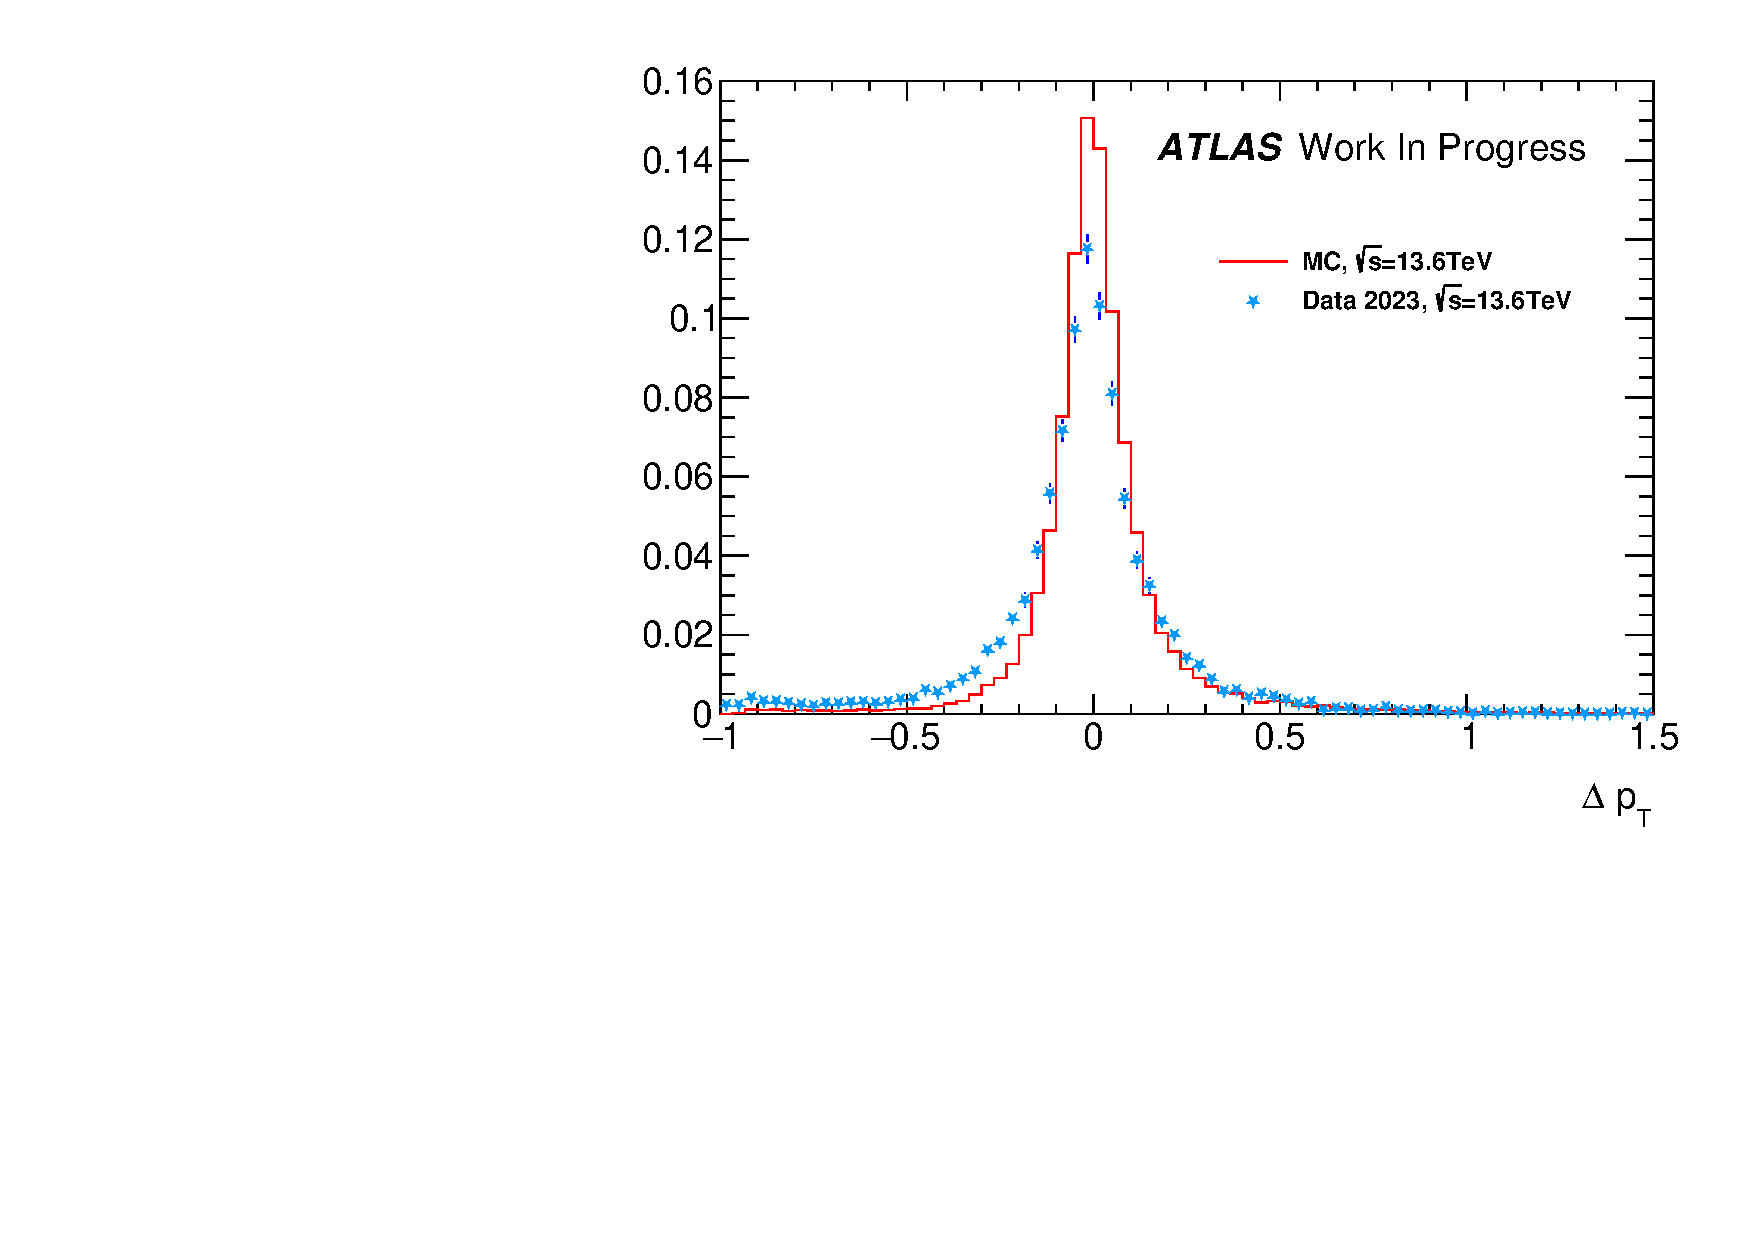
\includegraphics[clip, width=12cm]{fig/5/ptresidual_NSW.pdf}
    \caption{L2MuonSAでNSWを用いた時の$\pt$~residual}
    \label{fig:ptresidualDataMC}
\end{figure}

\begin{figure}[H]
    \centering
    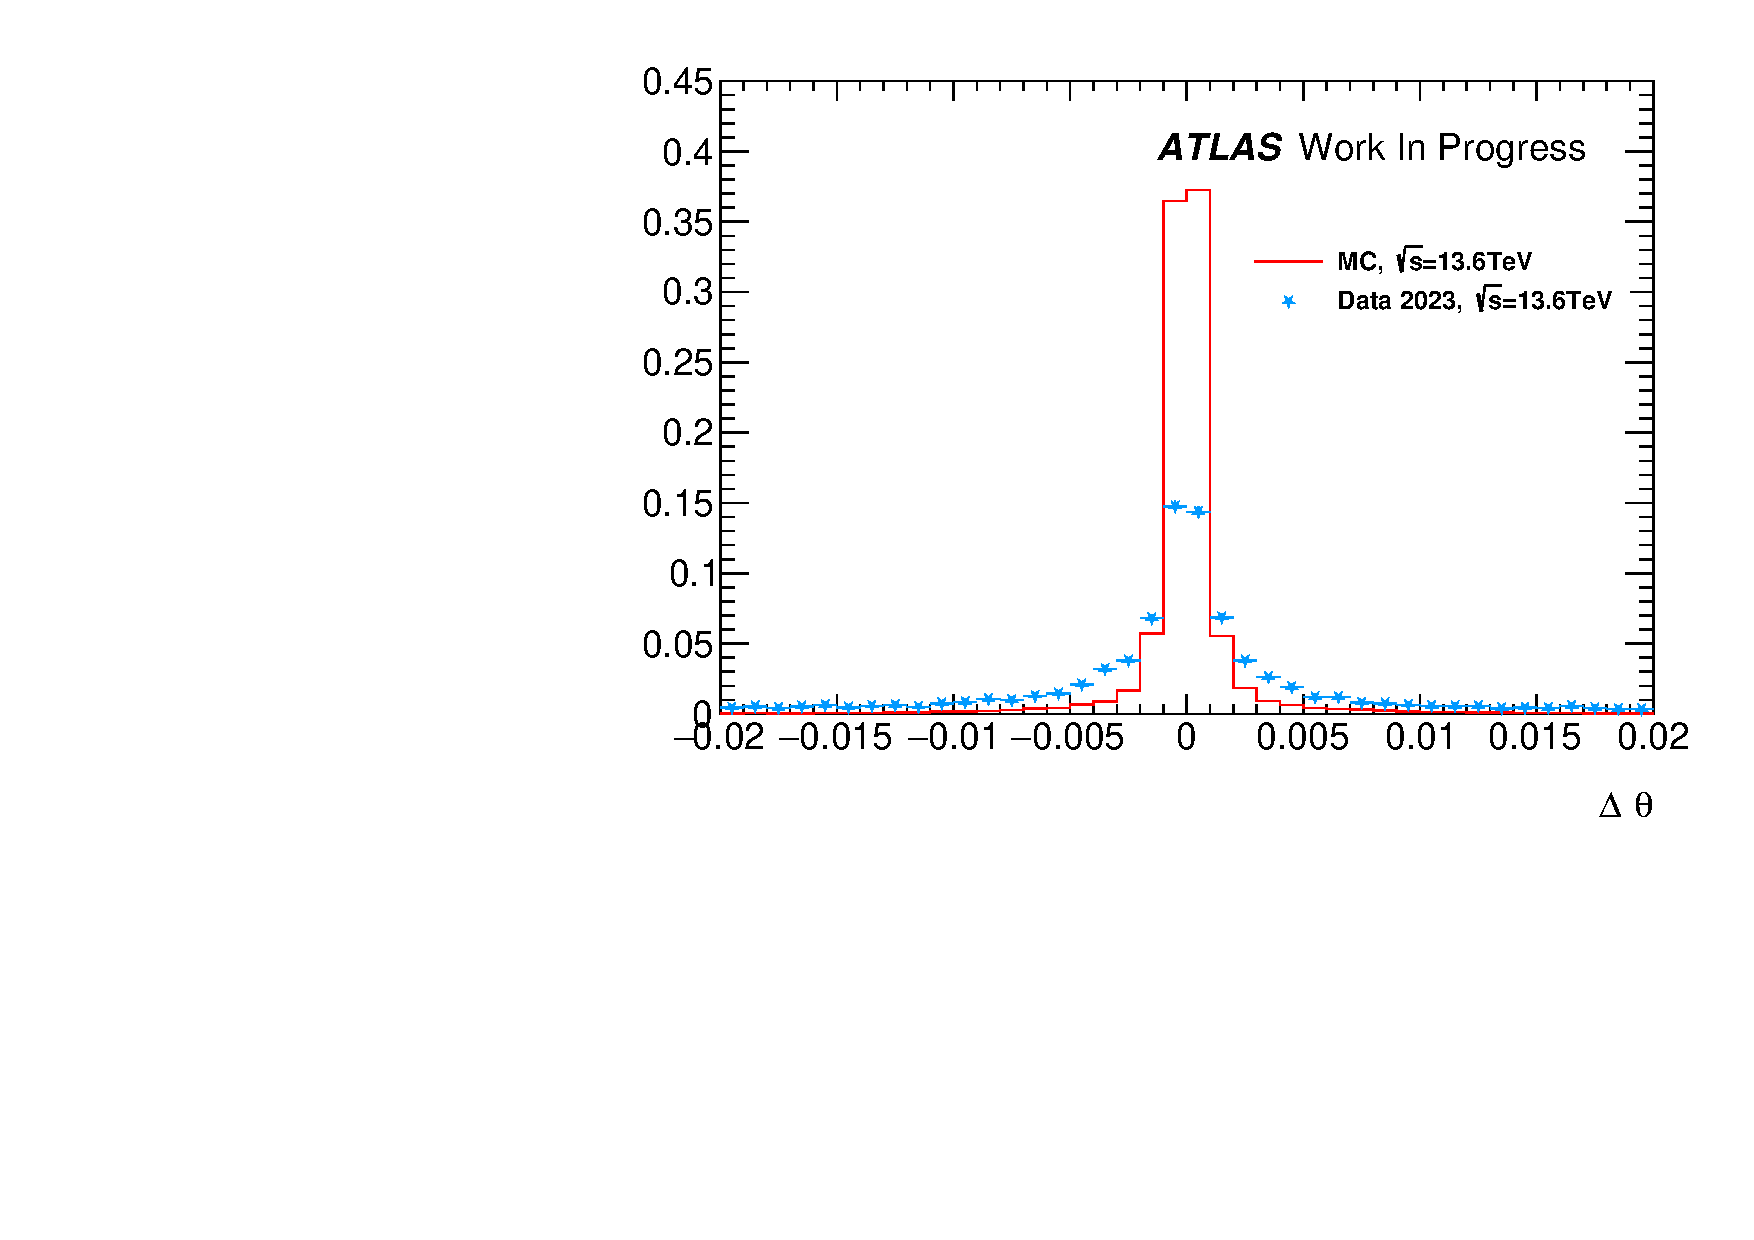
\includegraphics[clip, width=12cm]{fig/5/deltaTheta_NSW.pdf}
    \caption{L2MuonSAでNSWを用いた時の$\Delta \theta$}
    \label{fig:deltaThetaDataMC}
\end{figure}

\begin{figure}[H]
    \centering
    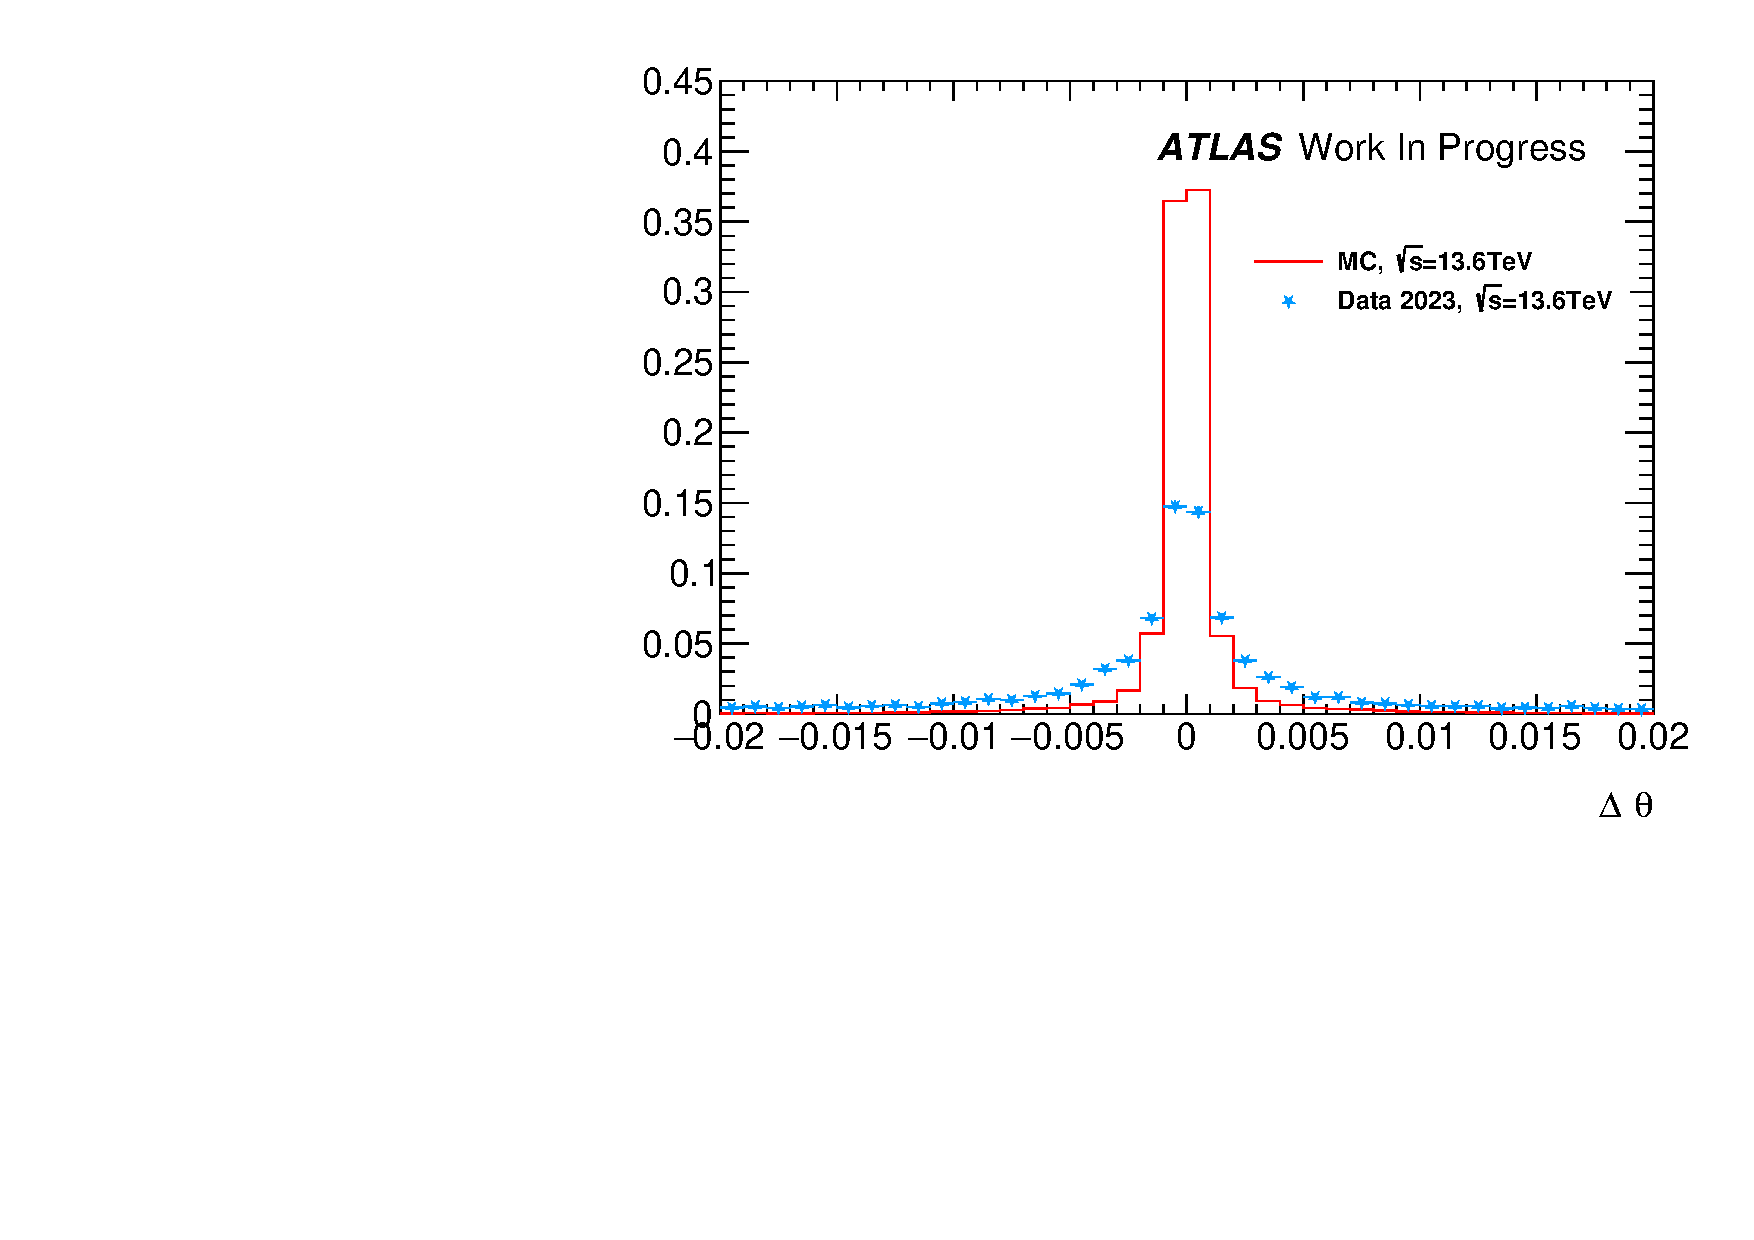
\includegraphics[clip, width=12cm]{fig/5/deltaTheta_NSW.pdf}
    \caption{L2MuonSAでNSWを用いた時の$\Delta \theta$}
    \label{fig:ptresidualAlphaBeta}
\end{figure}


図~\ref{fig:ptresidualDataMC}より、Run-3実データに対して~L2MuonSAで~NSWを$\pt$再構成に用いると、シミュレーションでの結果よりも$\pt$~residualが悪くなるということがわかる。
同様に、図~\ref{fig:deltaThetaDataMC}からデータでの$\Delta \theta$分布もピークの高さが低くなり、広がりが増えていることから~L2MuonSAでの部分飛跡再構成の精度がシミュレーションよりも悪くなっていることがわかる。

また図~\ref{fig:ptresidualAlphaBeta}から$p_{\rm{T, \alpha}}$の方が$p_{\rm{T, \beta}}$よりも$\pt$~residualがいい、つまり~L2MuonSAでの$\pt$再構成にインナーステーションの~NSWの情報を組み合わせて行う場合よりも、ミドルステーションとアウターステーションの情報のみで$\pt$再構成を行う方が$\pt$再構成の精度がいいということがわかった。

実データで$\pt$分解能が悪くなる原因として、~NSWの~SPを再構成する際に~MMのヒットを十分使えていないことが考えられる。
SP再構成に用いた~sTGC~stripと~MMのヒットの個数を以下に示す。

\begin{figure}[H]
  \begin{minipage}[b]{0.48\linewidth}
      \centering
      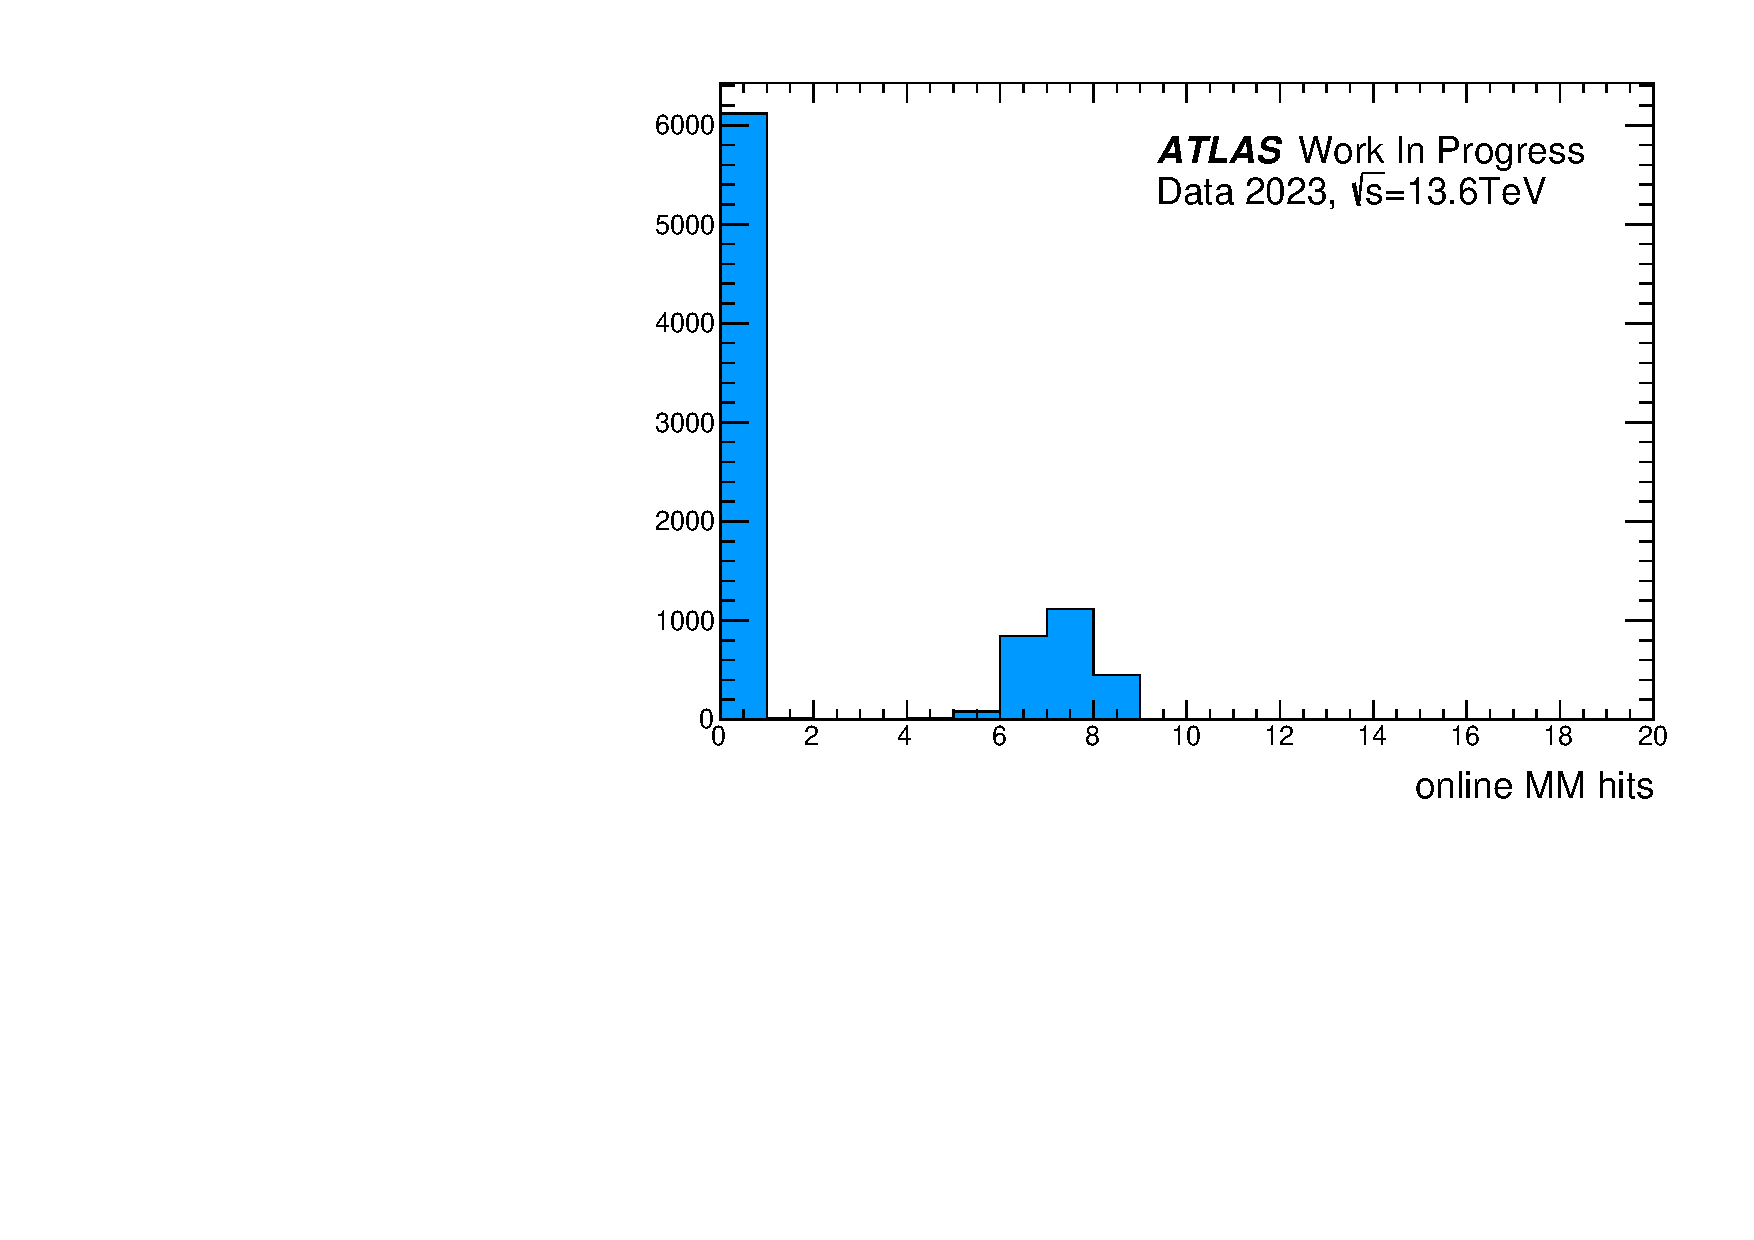
\includegraphics[clip, width=6.8cm]{fig/5/data_onlinemm.pdf}
      \subcaption{MMのヒットの個数}
      \label{fig:5-8-1}
  \end{minipage}
    \begin{minipage}[b]{0.48\linewidth}
      \centering
      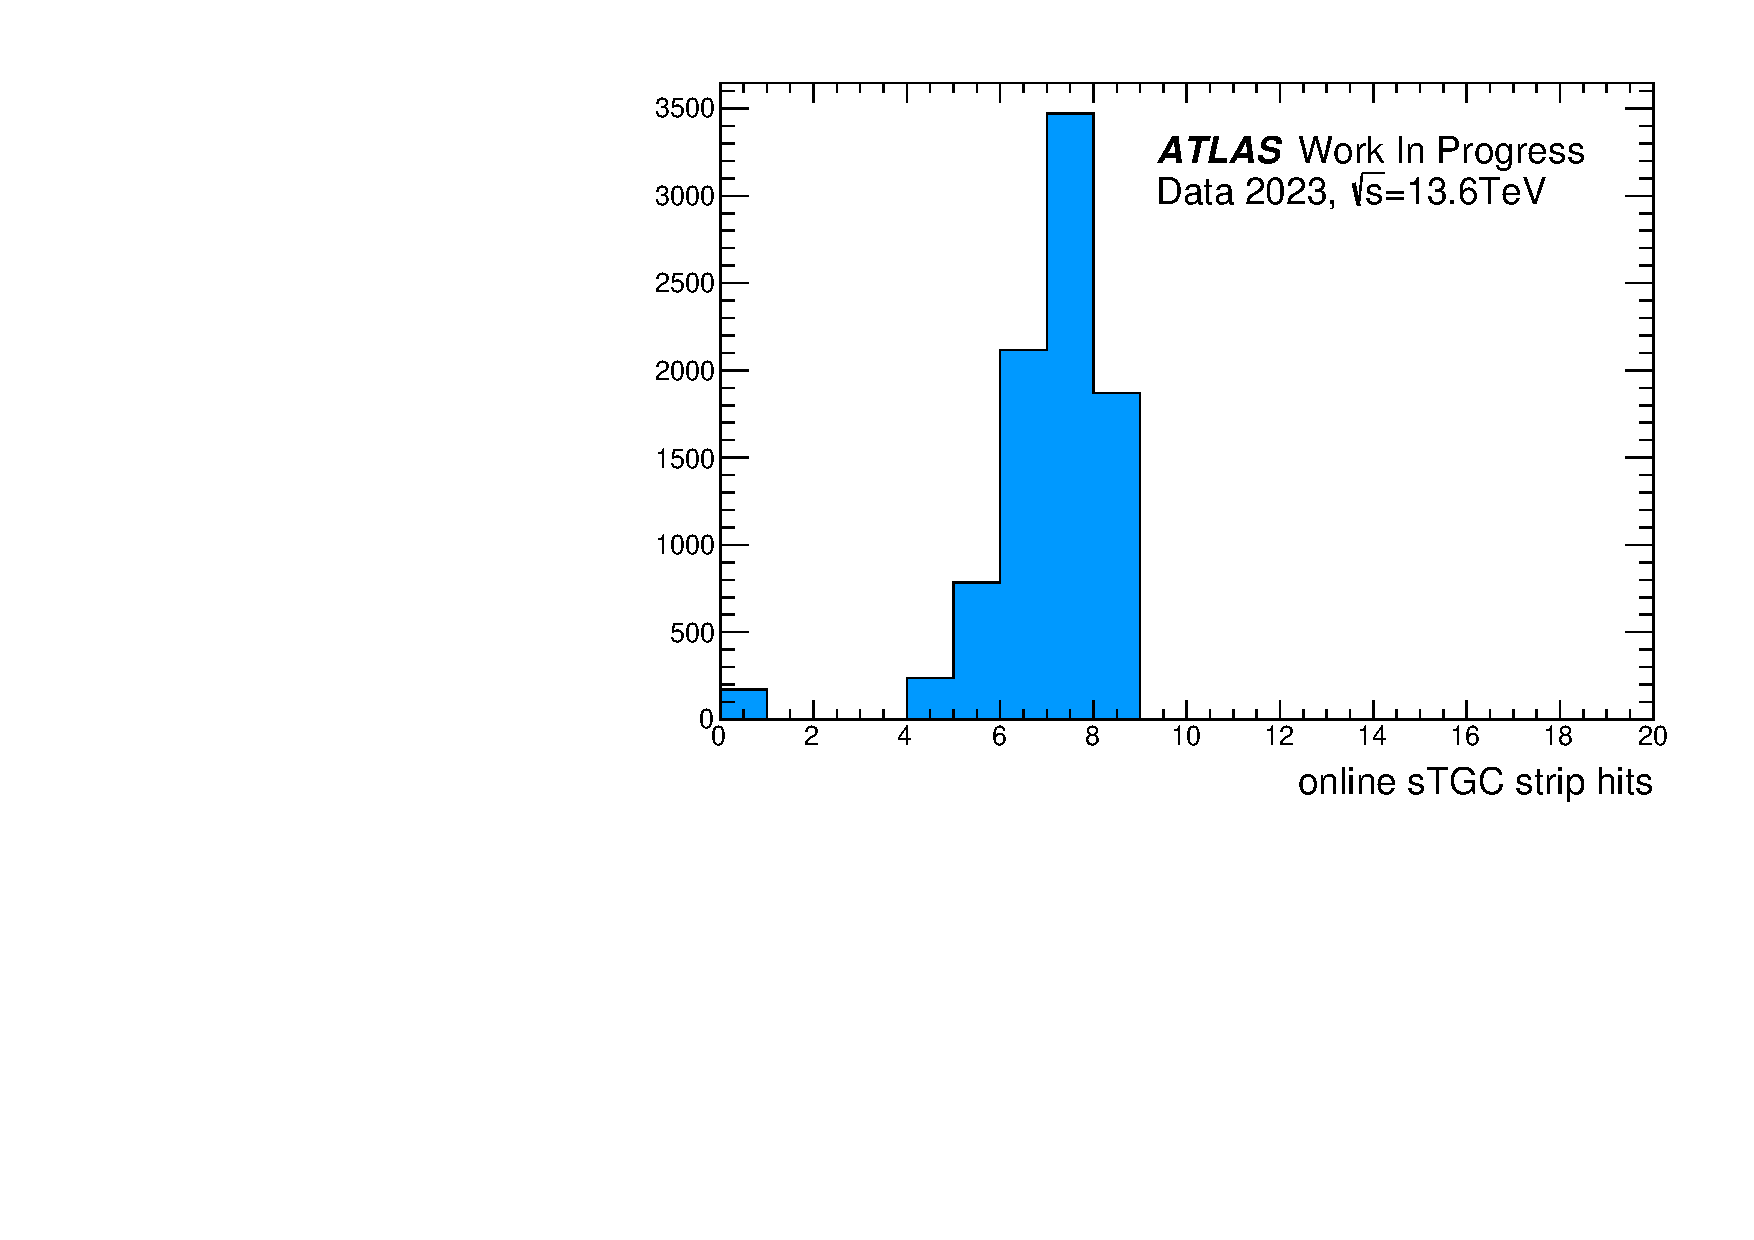
\includegraphics[clip, width=6.8cm]{fig/5/data_onlinestgceta.pdf}
      \subcaption{sTGCのヒットの個数}
      \label{fig:5-8-2}
  \end{minipage}
  \caption{Run-3実データにおけるNSWでの~SP再構成に用いたsTGC~stripと~MMのヒットの個数}
\end{figure}

第2章~\ref{section2-2-5}で述べたように、sTGCと~MMはそれぞれ8層ずつ設置されているので、ヒット選択アルゴリズムによって選ばれ~SPの再構成に用いるヒットの数は8個あたりにピークがあることが理想である。

しかし上図において~NSWの~SP再構成に用いた~sTGCのヒット数は7個あたりにピークがあるのに対して、MMのヒット数はほとんどのイベントで0個であり、NSWで~SPを再構成する際にほとんど~MMのヒットを使えていないことがわかった。

一方でシミュレーションでの~SP再構成に用いたヒット数の分布は図~\ref{fig:5-9}で示すように、~MMのヒット数は8個のところにピークがありSP再構成に~MMのヒットを十分使えているということがわかった。

\begin{figure}[H]
  \begin{minipage}[b]{0.48\linewidth}
      \centering
      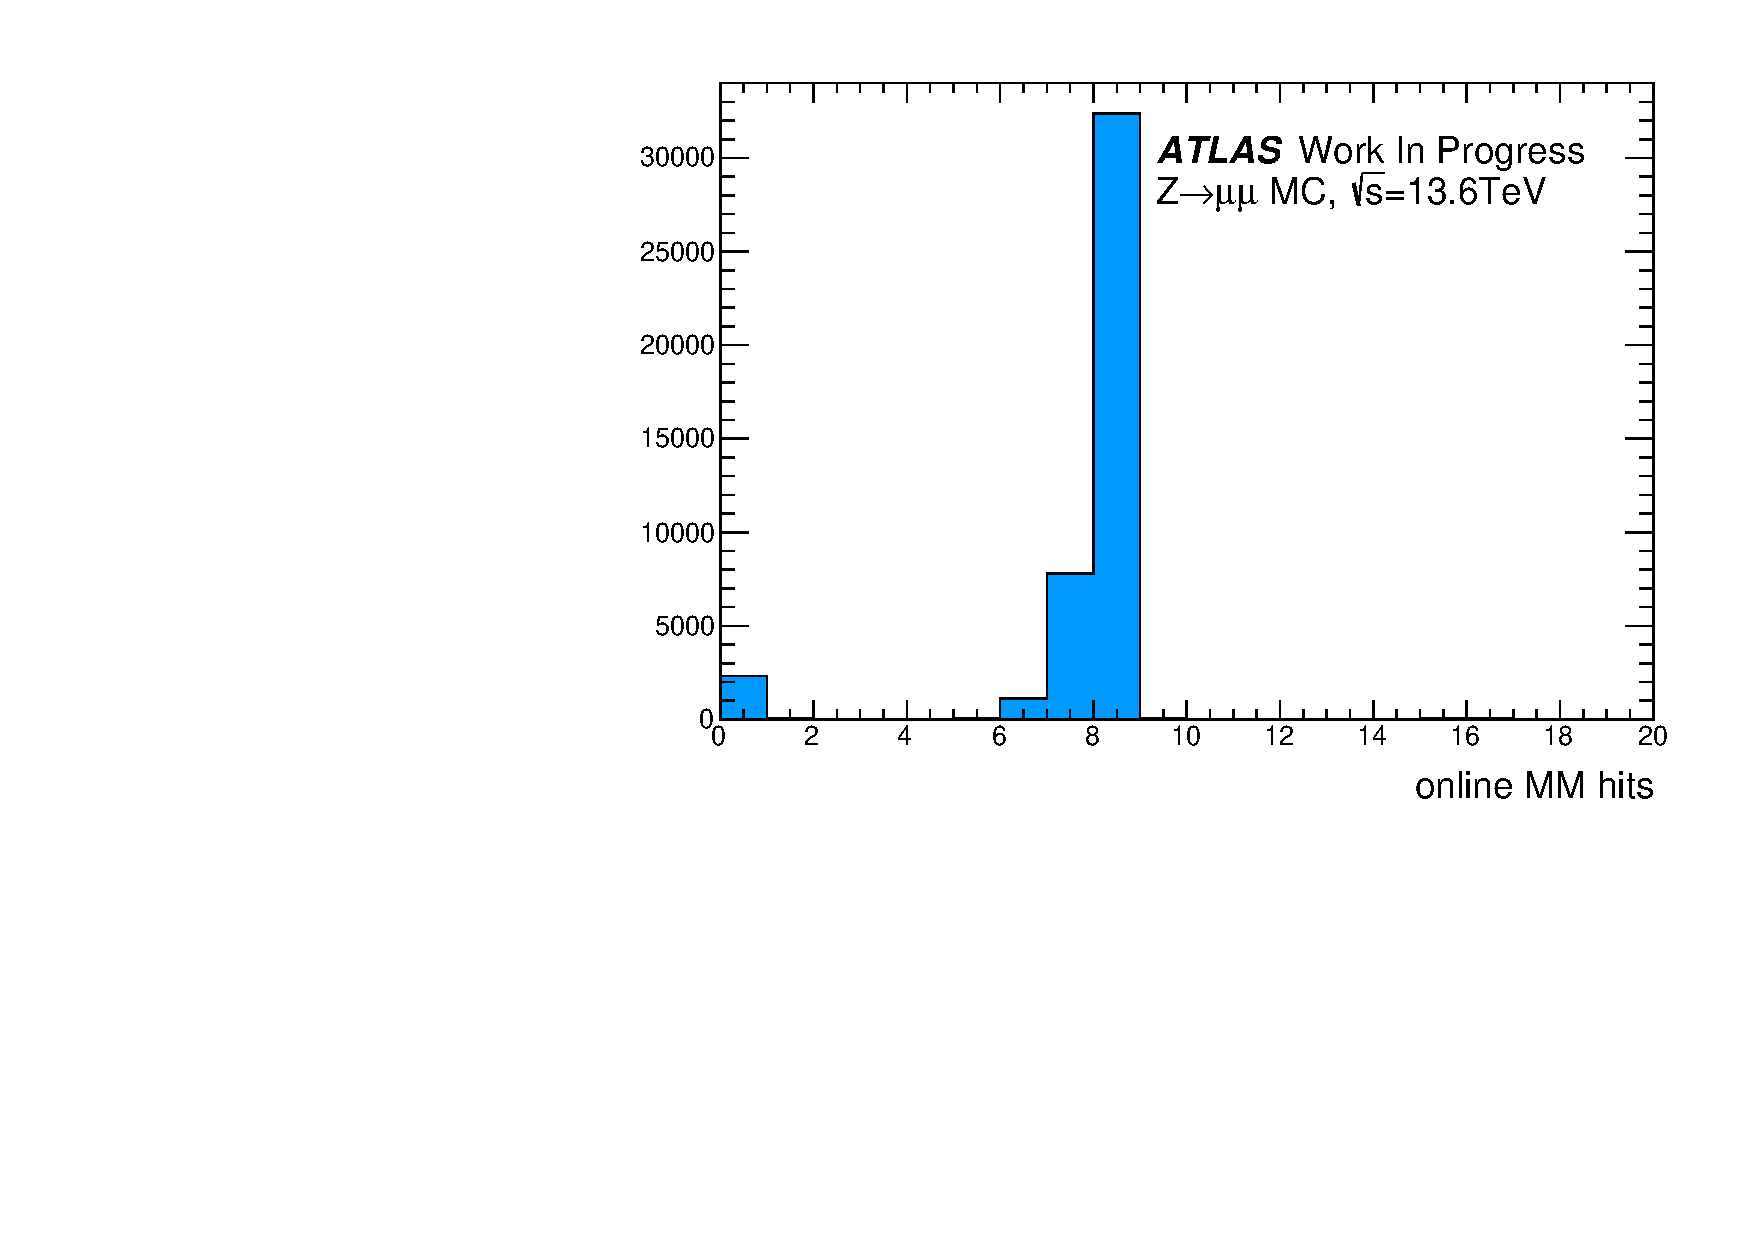
\includegraphics[clip, width=6.8cm]{fig/5/MC_onlinemm.pdf}
      \subcaption{MMのヒットの個数}
      \label{fig:5-9-1}
  \end{minipage}
    \begin{minipage}[b]{0.48\linewidth}
      \centering
      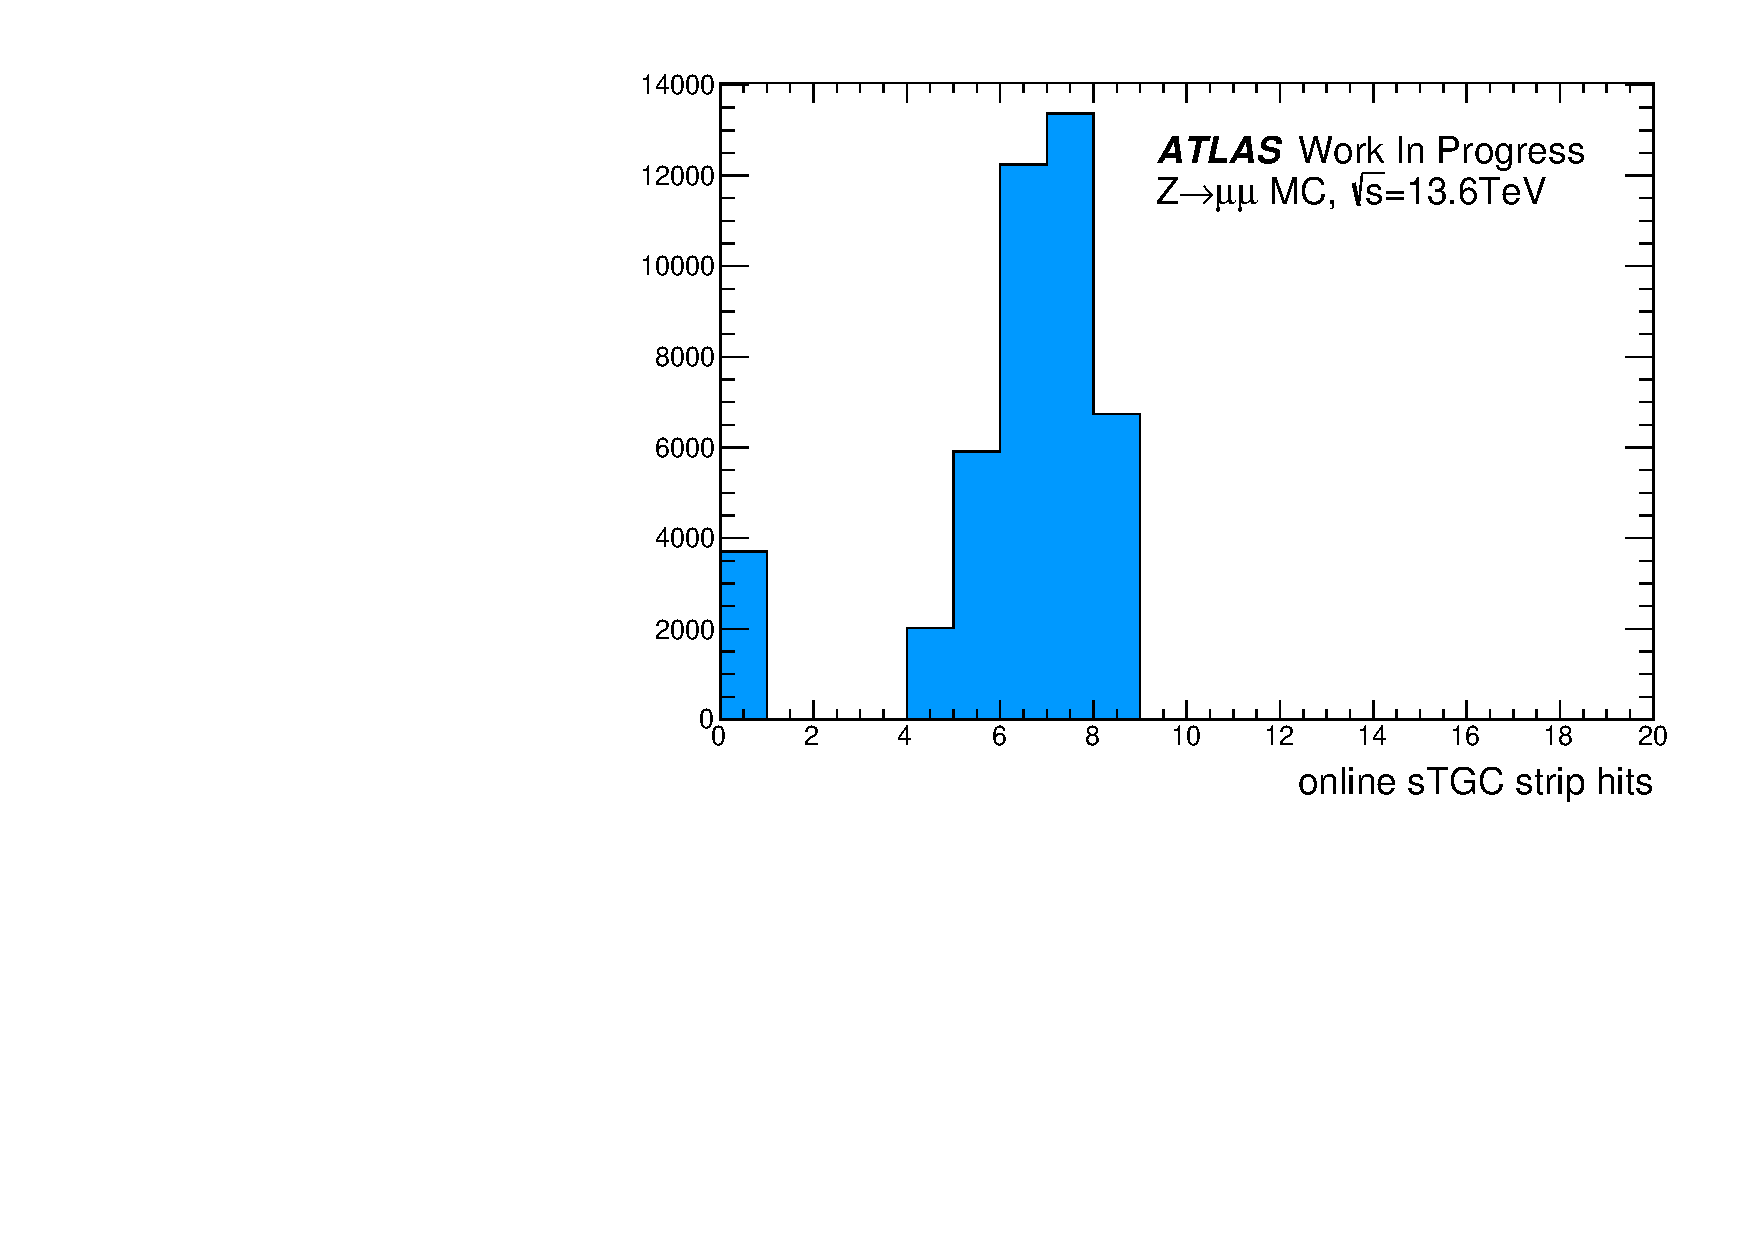
\includegraphics[clip, width=6.8cm]{fig/5/MC_onlinestgceta.pdf}
      \subcaption{sTGCのヒットの個数}
      \label{fig:5-9-2}
  \end{minipage}
  \caption{シミュレーションにおけるNSWでの~SP再構成に用いたsTGC~stripと~MMのヒットの個数}\label{fig:5-9}
\end{figure}


実データにおいて~MMのヒットがほとんど使えていない原因としては、現在のアルゴリズムでは~MMのヒットを選ぶ際に真っ直ぐ並んでいることを強く要求しているが、Run-3では~MMのヒットが真っ直ぐ並んでいるイベントが少ないのでヒット選択アルゴリズムで選ばれておらず~SPの再構成に用いられていないことが考えられる。

Event~displayを作成して、NSWのヒット~(~sTGC~strip、MM)と~SPの傾きと切片、インナーステーションにおけるオフラインセグメントの様子を視覚的に確認した。
%eventNum:7882,9191

\begin{figure}[H]
  \begin{minipage}[b]{0.45\linewidth}
      \centering
      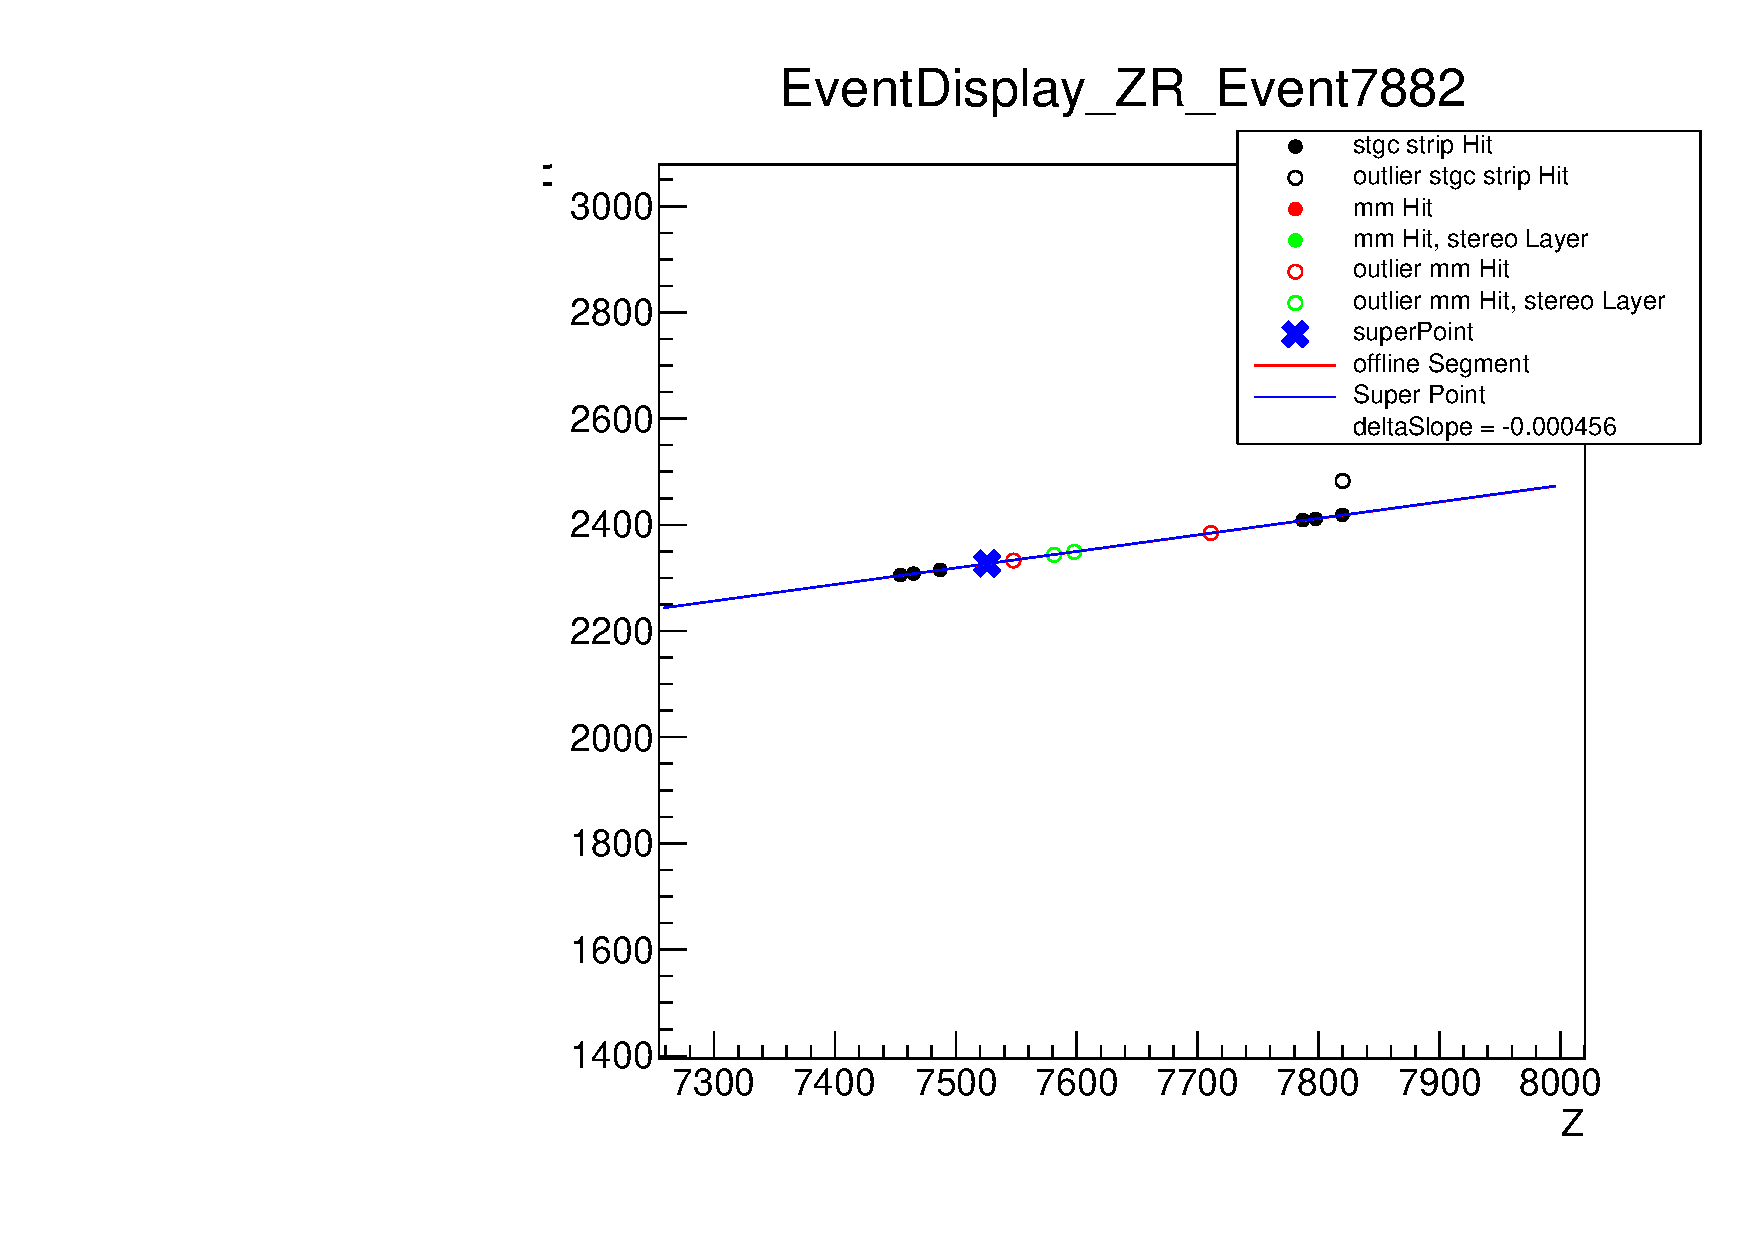
\includegraphics[clip, width=5.5cm]{fig/5/EventDisplay_7882_ZR_withMM.pdf}
      %\label{fig:5-10-1}
  \end{minipage}
    \begin{minipage}[b]{0.45\linewidth}
      \centering
      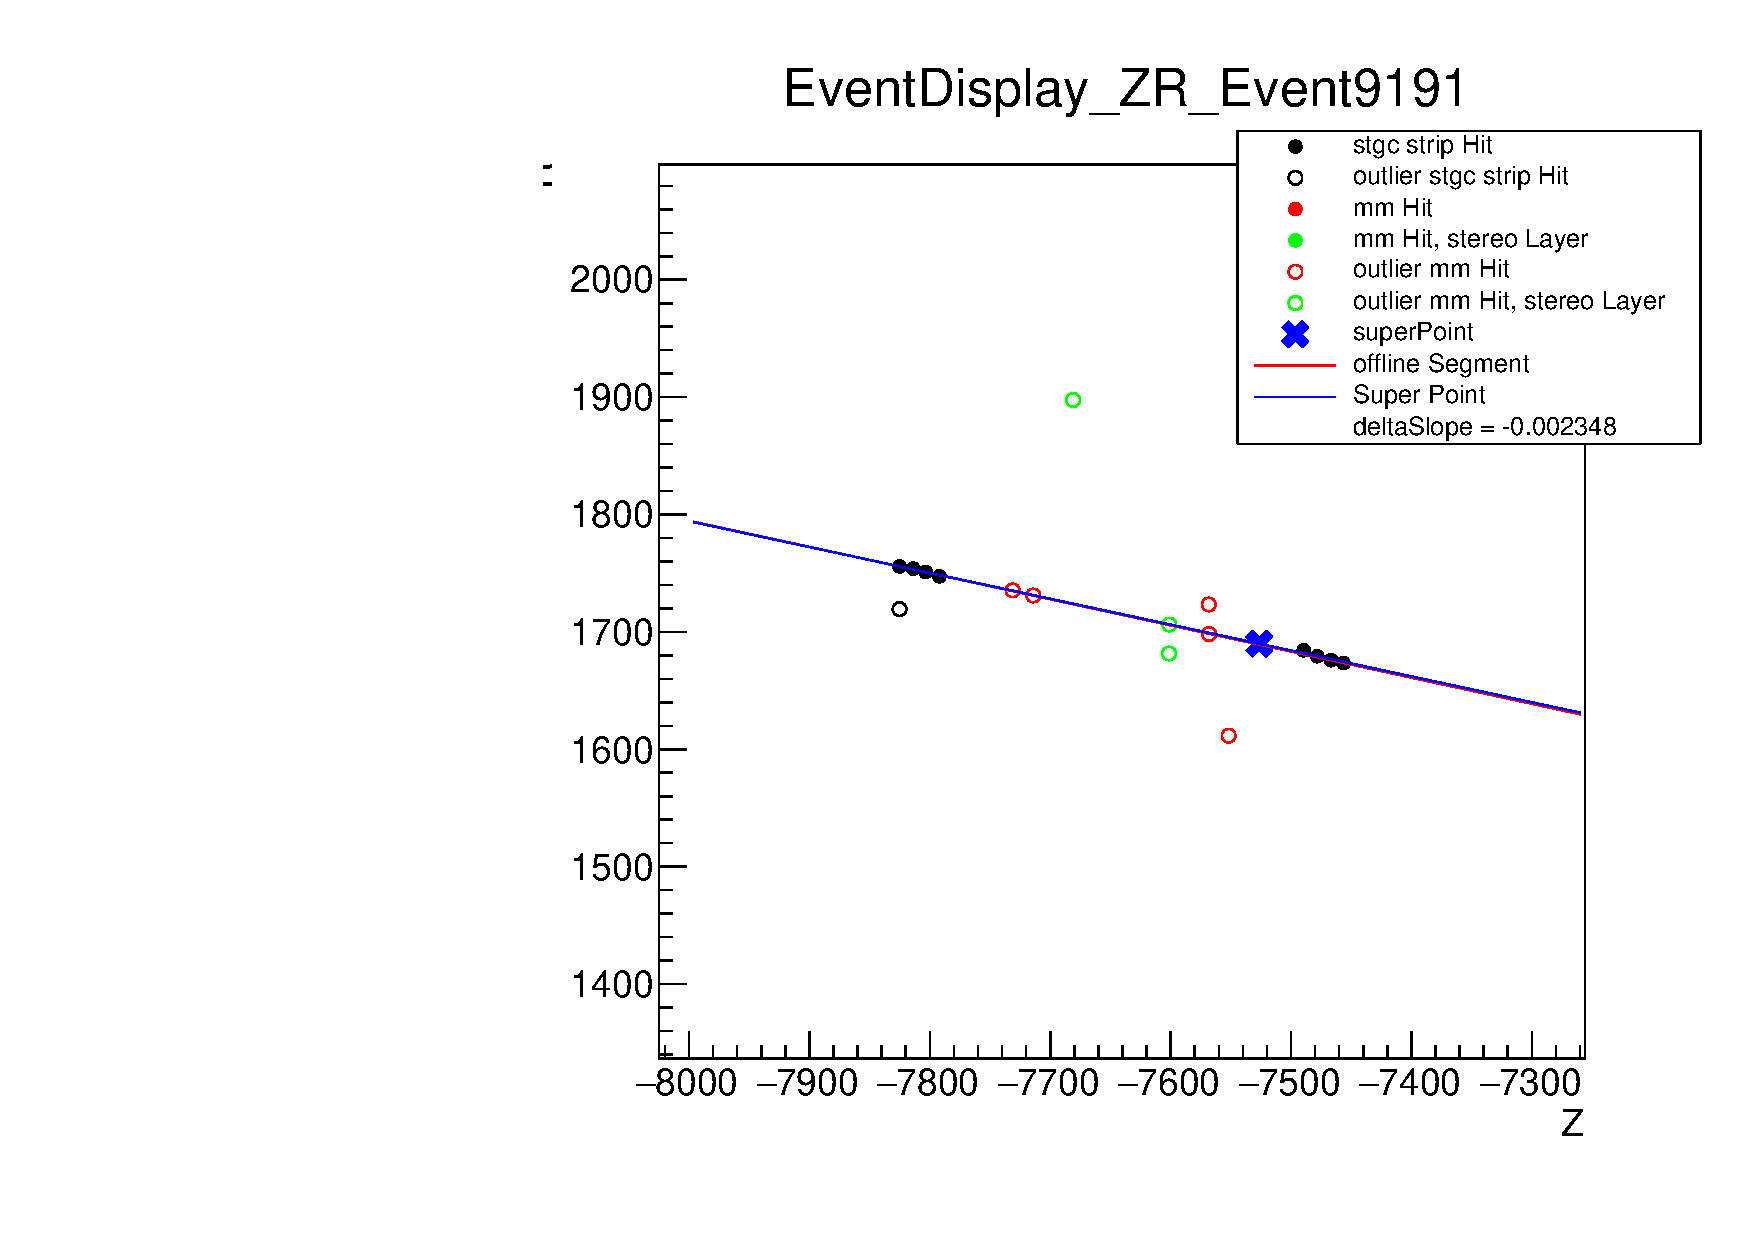
\includegraphics[clip, width=5.5cm]{fig/5/EventDisplay_9191_ZR_withMM.pdf}
      %\label{fig:5-10-1}
  \end{minipage}
  \caption{Event~displayでの~NSWのヒットと~SP、オフラインセグメントの様子}\label{fig:5-10}
\end{figure}

Event~displayで見てみると、NSWの~SPの傾きと切片から引いた直線の周りに~MMのヒットはあるが、ヒット同士が真っ直ぐ並んでいなく、また~MMは全部で8層あるがすべての層にヒットがなく~MMヒット選択アルゴリズムで選ばれていないということがわかった。


以下の分布は~NSWで~SPが作成されたときの、NSWの~SP再構成に使われたヒットの個数と、ミドルステーションから定義されたロード内にあるが~SPの再構成に使われなかったヒットの個数を~sTGCと~MMそれぞれについて示している。

\begin{figure}[H]
  \begin{minipage}[b]{0.48\linewidth}
      \centering
      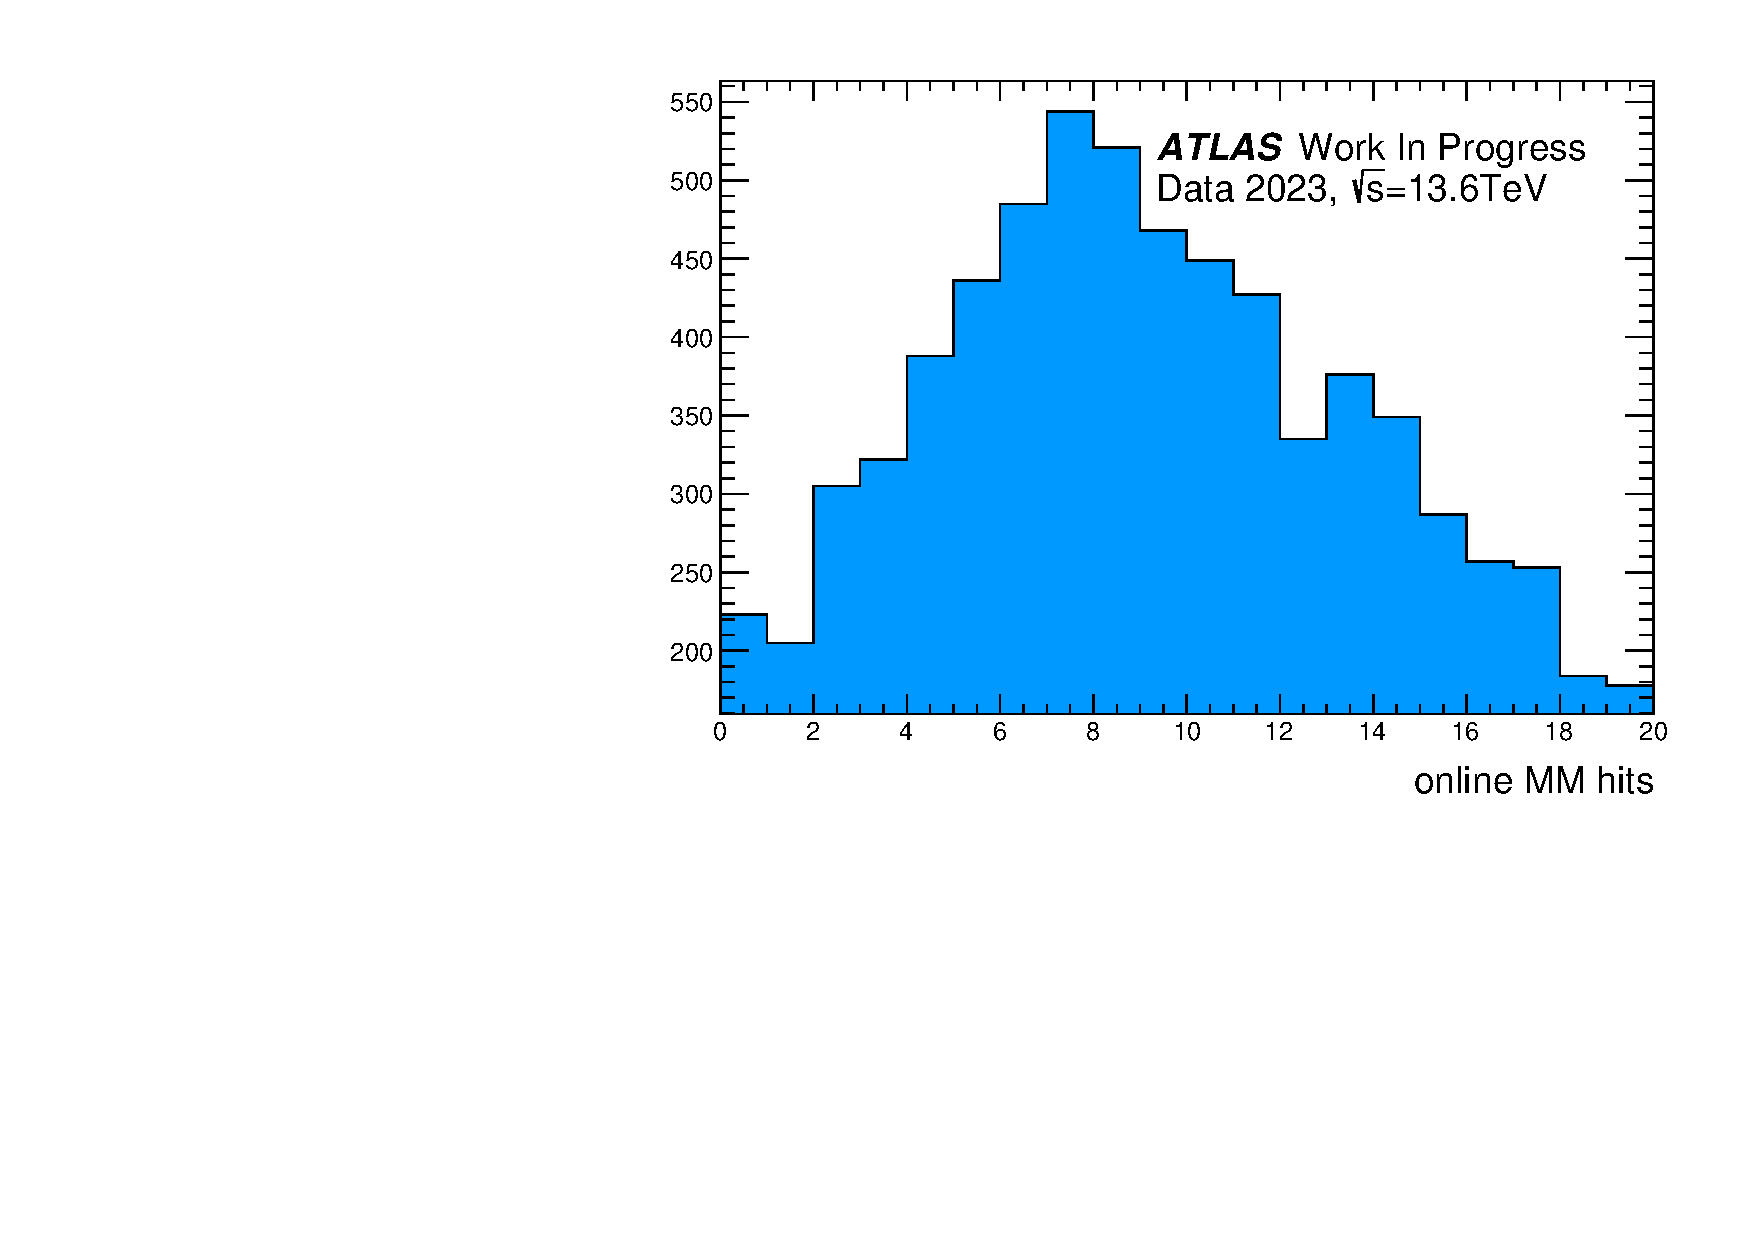
\includegraphics[clip, width=6.8cm]{fig/5/data_onlinemmIsoutlier.pdf}
      \subcaption{MMのヒットの個数}
      %\label{fig:5-11-1}
  \end{minipage}
    \begin{minipage}[b]{0.48\linewidth}
      \centering
      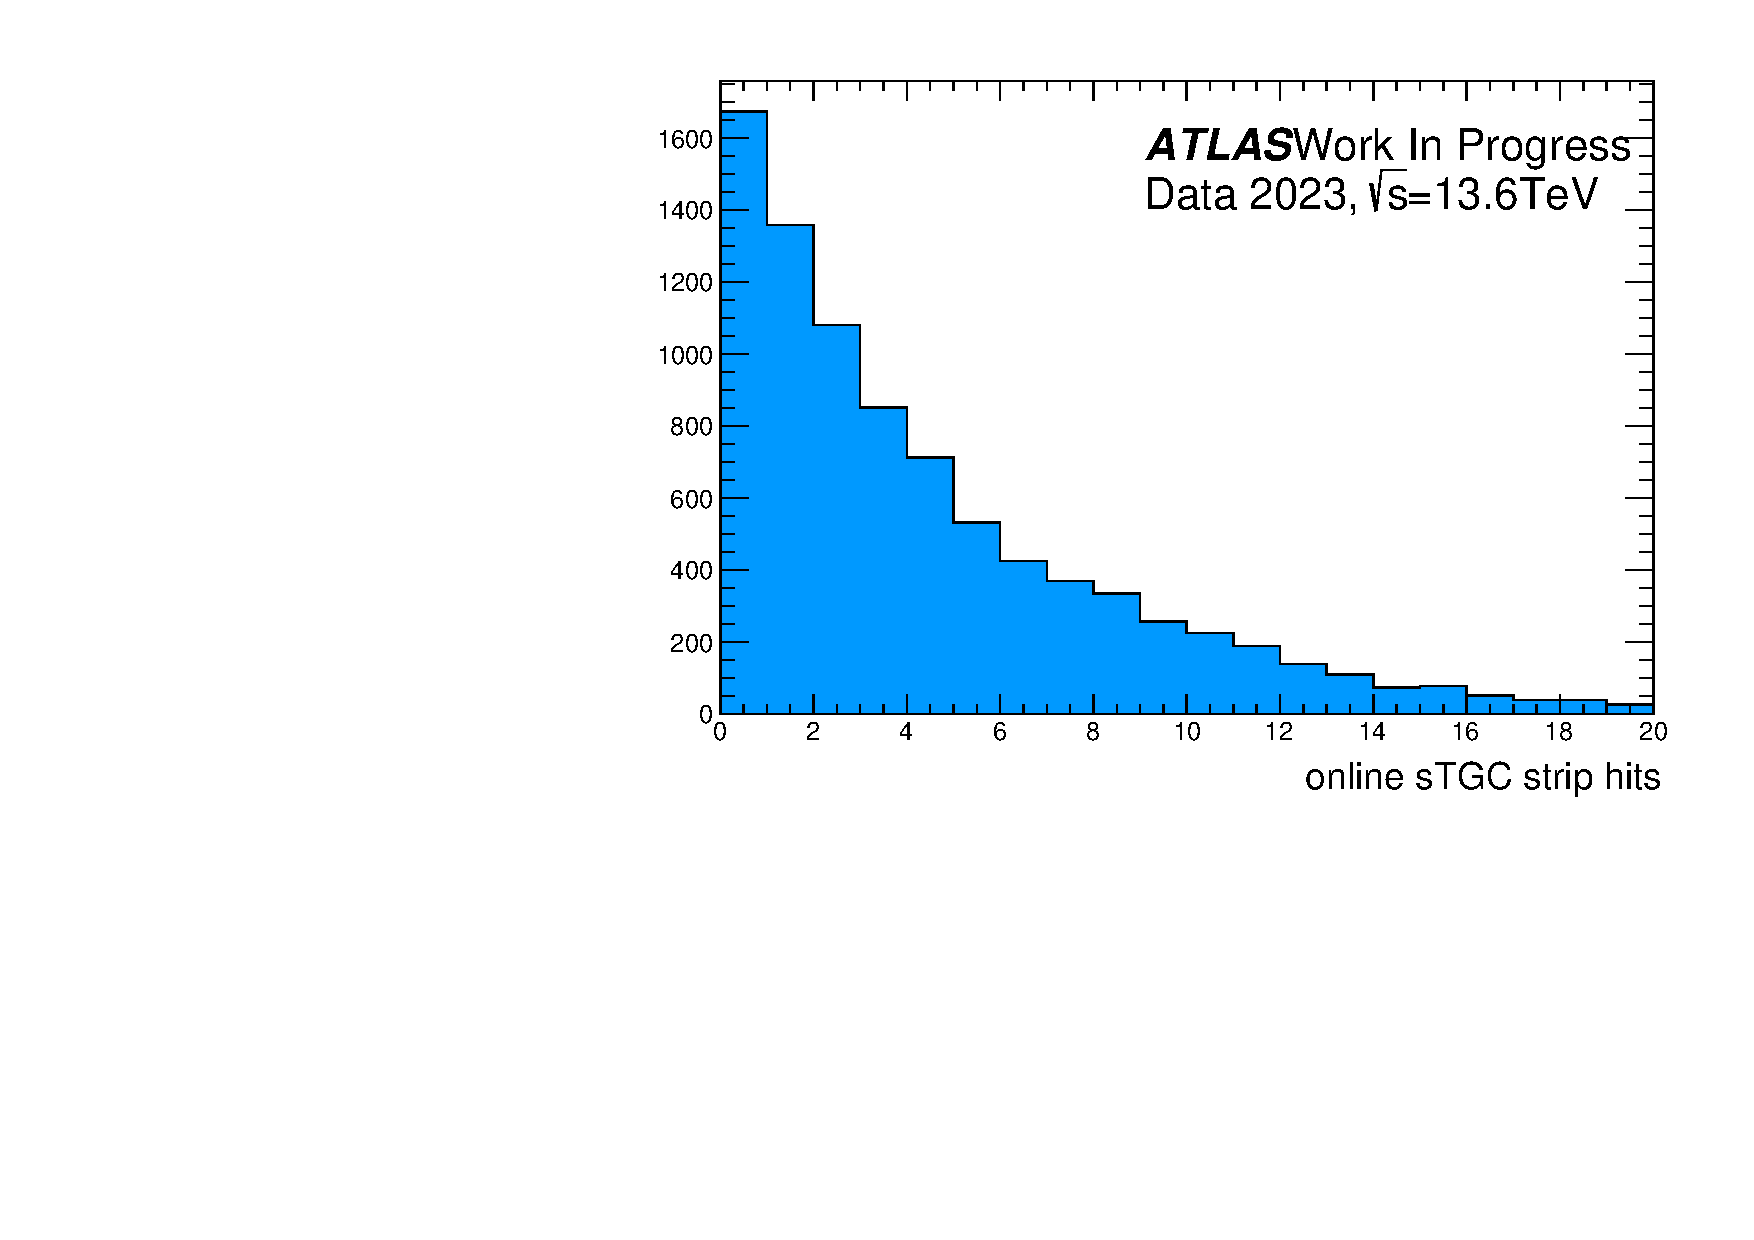
\includegraphics[clip, width=6.8cm]{fig/5/data_onlinestgcetaIsoutlier.pdf}
      \subcaption{sTGCのヒットの個数}
      %\label{fig:5-11-1}
  \end{minipage}
  \caption{ロード内にあるが~SPの再構成に用いられなかったヒットの個数}\label{fig:5-11}
\end{figure}

ほとんどのイベントで、MMのヒットはミドルステーションから引いたロード内にあるが、~SPの再構成に用いられていないということがわかった。

一方で図~\ref{fig:5-10}より~sTGCのヒットはきれいに直線で並んでおり8層のうちほとんどにヒットがあるということがわかる。そのため現行のヒット選択アルゴリズムで十分にヒットを選ぶことができている。
第5.1節~\ref{chapter5-1}で述べた通り、現行のヒット選択アルゴリズムでは~sTGC、MMはそれぞれ独立にヒット選択を行っている。現在L2MuonSAで用いているヒット選択アルゴリズムでは~sTGCのヒットは十分選ぶことができるが、MMに対しては十分選べない。

そこで新たに~MMのヒットが真っ直ぐ並んでいない場合や、ヒットがある層が少ない場合でも~SP再構成に用いることができるようなアルゴリズムを検討した。

\section{新たに検討した~NSWヒット選択アルゴリズム}\label{chapter5-4}
新たに検討したアルゴリズムの目的は、前の節で述べたように、MMのヒットがロード内に存在するが真っ直ぐ並んでいない場合やヒットがある層が少ない場合でも~NSWの~SP再構成に用いることである。

現行のヒット選択アルゴリズムで~sTGCのヒットは十分選べており、SPの直線の近くに~MMのヒットも多いことから現行のアルゴリズムで選ばれた~sTGCのヒットを用いて~MMのヒットを選び~SPの作成に用いることで$\pt$分解能の向上に繋がるのではないかと考えた。


検討したアルゴリズムの流れを以下に示す。
\begin{enumerate}
    \item まず現行のヒット選択アルゴリズムで~SP再構成をする際に選んだ~sTGCヒットに対して直線フィットを行い、この直線を中心とするロードを新たに定義する。
    \item 1で定義したロード内にある~MMのヒットを選ぶ。この際に同じ層にヒットがある場合も除外しない。
    \item 1で用いた~sTGCヒットと、2で選んだ~MMヒットに対して直線フィットを行い、新たな~SPの傾きと切片を定義する。
\end{enumerate}


\begin{figure}[H]
    \centering
    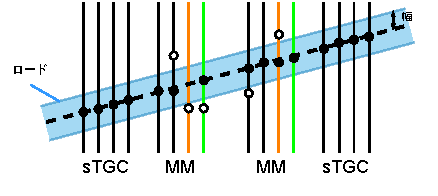
\includegraphics[clip, width=10cm]{fig/5/newHitSelectAlg.pdf}
    \caption{検討した~NSWヒット選択アルゴリズムの概要。MMの黒丸のヒットは~SP再構成に用いて、白丸のヒットは用いない。}
    \label{fig:5-12}
\end{figure}

sTGCのヒットから再定義したロードの幅については何パターンか変化させ、$\pt$~residualがどう変化するか試した。


\section{検討した~NSWヒット選択アルゴリズムの性能評価}\label{chapter5-5}